\section{Sum of Infeasibilities for Mode Sequences}
\label{sec:soi}

Alg.~\ref{alg:complete} is sound and complete. It returns \feas if and only if there is a feasible solution satisfying both the linear constraints and the precise one-hot constraints. However, since \convProc operates on convex relaxations and is unaware of the binary constraints, it can find spurious solutions that violate the binary constraints, leading to costly branching.
\begin{wrapfigure}{r}{0.25\textwidth}
\vspace{-4mm}
\centering
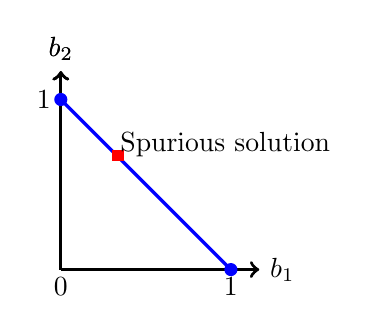
\begin{tikzpicture}[scale=0.72]
\draw[->, very thick] (0, 0) -- (3.5, 0) node[right] {$b_1$};
\draw[->, very thick] (0, 0) -- (0, 3.5) node[above] {$b_2$};
\draw[->, very thick] (0, 0) -- (0, 3.5) node[above] {$b_2$};
\draw[domain=0:3, very thick, variable=\x, blue] plot ({\x}, {3-\x});

%\draw[<-, very thick, dashed] (0.1, 2.6) -- (0.75, 1.95);
%\draw[->, very thick, dashed] (1, 1.8) -- (2.6, 0.2);


\node at (0, -0.3) {0};
\node at (3, -0.3) {1};
\node at (-0.3, 3) {1};
\draw[draw=red, fill=red] (0.92,1.92) rectangle ++(0.18,0.18);
\node at (2.9, 2.2) {Spurious solution};
\filldraw[blue] (0, 3) circle (3pt);
\filldraw[blue] (3, 0) circle (3pt);
\end{tikzpicture}
\caption{Solutions found by convex solver can be spurious.}
\label{fig:onehot}
\vspace{-2mm}
\end{wrapfigure}

Fig.~\ref{fig:onehot} illustrates this phenomenon for a one-hot constraint with two modes (represented by $b_1$ and $b_2$). In its convex relaxation, $(b_1, b_2)$ can lie anywhere on the line segment in the figure.% Therefore, it is possible that the LP solver finds a feasible solution for the convex relaxation that does not satisfy the precise constraint (e.g., the squared point).

Ideally, we want the convex optimization procedure to be more aware of the precise one-hot constraints so that it can avoid branching. We propose to achieve this by ``softly'' guiding the convex procedure with a cost function \soi, called the sum-of-infeasibilities, that represents the violation of the one-hot constraints. Minimizing \soi over the convex relaxation naturally leads to a feasible solution that satisfies both the convex relaxation and the precise integral requirements. We next introduce our \soi function for one-hot constraints, consider the challenge of its minimization, and present a stochastic local search solution.

\subsection{The Sum of Infeasibilities}
As mentioned above, in convex optimization, a sum-of-infeasibilities function represents how much the current solution violates the convex constraints. Here, we build on this idea by introducing a cost function $\soi$, which computes the sum of errors introduced by the convex relaxation of one-hot constraints.\footnote{Similar ideas have been used to reason about different types of non-linear constraints in a different setting~\cite{wu2022efficient}.}
$\soi$ needs to meet the following condition:
\begin{condition}
  \label{cond:soi}
  Given a set of linear constraints $\C$ and a set of one-hot constraints $\O$ defined over variables $\realvars$, a solution $\alpha$ is feasible for $\phi:= \C\cup \O$ iff
  $\alpha$ is a feasible solution to $\rlx{\phi}$ and $\soi(\alpha) \leq 0$. \label{condition:soi}
\end{condition}
If Condition~\ref{cond:soi} is met, then feasibility of $\phi$ reduces to
the following minimization problem:
\begin{equation}
  \begin{aligned}
    \minimize_{\realvars} \quad &\soi(\realvars)\\
    \textrm{subject to} \quad &\rlx{\phi}
  \end{aligned}
  \label{eq:min}
\end{equation}


To formulate \soi for a problem with one-hot constraints, we first define the error in a single one-hot constraint $\onehot(\binvars)$ as:
%\begin{equation}
$\vio(\binvars) = 1 - \max(\binvars)$.
%\label{eq:vio}
%\end{equation}
Note that $\vio(\binvars)$ subject to $\rlx{o}$ is non-negative and $\vio(\binvars) = 0$ iff $o$ is satisfied.
We  define $\soi$ as the sum of errors in each individual one-hot constraint:
\begin{equation}
  \soi = \sum_{\onehot(\binvars) \in \O}\vio(\binvars)
  \label{eq:soi}
\end{equation}

\begin{theorem}
$\soi$ as given by~\eqref{eq:soi} satisfies Condition \ref{cond:soi}.
\end{theorem}

In particular, the minimum of $\soi$ is 0 and achieved if and only if $\max(\binvars)=1$ for each one-hot constraint $\onehot(\binvars)$. 

Now, observe that:
\begin{align}
  \soi &= \sum_{o(\binvars) \in \O}\vio(\binvars) \nonumber= \sum_{o(\binvars) \in \O}(\min_{b\in\binvars}(1 - b)) \nonumber\\
   &= \min\Big(\big\{ f \mid f = \sum_{o(\binvars) \in \O} (1 - b_i), \quad b_i \in \binvars \big\}\Big).
  % = \min(S_f)
  \label{eq:rearrange}
\end{align}
Thus, $\soi$ is the minimum over a set, which we denote $\soiset$, of linear functions. Although $\soi$ is concave piecewise-linear and cannot be directly minimized with convex optimization, we could minimize each individual function $f\in \soiset$ and take the minimum over all functions. Notice that each linear function in $\soiset$ has a semantic meaning: it corresponds to a particular mode sequence, i.e., a choice of modes at each time step. For notational convenience, we define $\costOf(f,\phi)$ to be the minimum of $f$ subject to $\phi$. Thus, the minimization problem \eqref{eq:min} can be restated as searching for a mode sequence $f\in \soiset$, where $\costOf(f,\rlx{\phi})$ is minimal.

\subsection{Minimizing the SoI with MCMC Sampling \label{subsec:minSOI}}
In the worst case, minimizing \soi requires enumerating and minimizing each mode sequence. In practice, the search can terminate once a mode sequence $f$ is found such that $\costOf(f,\rlx{\phi}) = 0$. A local search procedure that ``greedily'' navigates towards the minimum can be used to search for such mode sequence.  One such method is \emph{Markov chain Monte Carlo} (MCMC)~\cite{mcmc-1}, which can be viewed as a class of intelligent hill-climbing algorithms robust against local optima. In our context, MCMC can be used to generate a chain of mode sequences $f_0, f_1, f_2... \in \soiset$, with the desirable property that in the limit, the sampled mode sequences are more frequently from the minimum region of $\costOf(f,\rlx{\phi})$.

We use the Metropolis-Hastings (M-H) algorithm~\cite{mh}, a widely applicable MCMC method, to construct the sequence. The algorithm maintains a current mode sequence $f$ and proposes to replace $f$ with a new mode sequence $f'$. The proposal comes from a \emph{proposal distribution} $q(f' | f)$ and is accepted with a certain \emph{acceptance probability} $m(f{\rightarrow}f')$. If the proposal is accepted, $f'$ becomes the new current mode sequence. Otherwise, another proposal is considered. This process is repeated until one of the following scenarios happen:
1) a mode sequence $f$ where $\costOf(f,\rlx{\phi}) = 0$ is found;
2) a predetermined computational budget is exhausted; 
3) all possible mode sequences have been considered.
%The last scenario rarely happens unless the space of possible mode sequences is small.

In order to employ the algorithm, we transform $\costOf(f,\rlx{\phi})$ into a probability
distribution $p(f)$ using a common method~\cite{mcmc}: $p(f) \propto \exp(-\beta \cdot \costOf(f,\rlx{\phi}))$,
where $\beta$ is a configurable parameter. We use the following acceptance probability
(often referred to as the \emph{Metropolis ratio})~\cite{mcmc}:
$m(f{\rightarrow}f') = \min(1, \frac{p(f')}{p(f)})$.

Importantly, under this acceptance probability, \textit{a proposal reducing the value of the cost function is always accepted, while a proposal that does not may still be accepted}
(with a probability that is inversely correlated with the increase in the cost). This means that the algorithm always greedily moves to a lower-cost mode sequence whenever it can, but it also has an effective means for escaping local minima.

%Since the sample space is finite, as long as the proposal strategy is \emph{ergodic} (i.e., capable of transforming any mode sequence to any other), we will \emph{almost surely} sample every mode sequence in the limit and therefore the procedure is probablistically approximately complete~\cite{hoos2015stochastic}. However, this is only of theoretical interests because our goal is to quickly find feasible mode sequence rather than ensuring completeness, which can be enabled by embedding the M-H algorithm in an exhaustive search shell like Alg.~\ref{alg:complete}.

\subsection{Stochastic Optimization for One-Hot Constraints}

\begin{algorithm}[t]
\small
\begin{algorithmic}[1]
\State {\bfseries Input:} $\C$, $\O$, $\E$
\State {\bfseries Output:} \feas/\infeas, feasible solution $\alpha$, theory lemmas $\L$ 
\State {\bfseries Parameters:} Sampling budget $T$ 
\Function{\deepsoiT}{$\C,\O, \E$}
\State $r, \alpha_0, \L \mapsto \convProc(\C\cup\rlx{\O})$
\If{$r = \infeas \lor \alpha_0\models \C\cup \O$} {\bf return} $r, \alpha_0, \L$
\EndIf
\State $k,f \mapsto 0, \initialCost(\alpha_0, \O)$ \label{line:initsoi}
\State $\alpha, c \mapsto \convOptProc(f, \C\cup\rlx{\O})$
\State {$\L \mapsto \{f > 0\}$}
\While{$c > 0 \land \neg \func{exhausted}() \land k < T$} 
\State $f' \mapsto \propose(f, \alpha, \E \cup \neg\prop(\L))$ \label{line:proposesoi}
\State $\alpha', c' \mapsto \convOptProc(f', \C\cup\rlx{\O})$
\If {$c' > 0$} {$\L \mapsto \L \cup \{f' > 0\}$}
\EndIf
\If {$\accept(c,c')$} $f,c, \alpha \mapsto f', c', \alpha'$
\Else {$\ k \mapsto k + 1$}
\EndIf
\EndWhile
\If {$\func{exhausted}() \land c > 0$} 
\State {\bf return} $\infeas, \alpha, \L$
\Else
\State {\bf return} $\feas, \alpha, \L$
\EndIf
\EndFunction
\end{algorithmic}
\caption{The \deepsoi procedure \label{alg:stoc}}
\end{algorithm}

The stochastic optimization procedure \deepsoi is shown in Alg.~\ref{alg:stoc}. It takes as input a set of linear constraints $\C$ and a set of one-hot constraints $\O$ and stochastically searches for a feasible solution to $\phi:= \C\cup\O$. It is intended as a drop-in replacement of the \convProc method in Line~\ref{line:checkconv} of Alg.~\ref{alg:complete} in order to more efficiently find solutions that satisfy not only the convex relaxation but also the binary constraints. Concretely, we will replace Line~\ref{line:checkconv} with 
\[
r, \alpha, \L \mapsto \deepsoi(\C\cup\D, \O, \E)
\]

\deepsoi follows the standard two-phase convex optimization approach. 
Phase I (Lines 5-6) finds a feasible solution $\alpha_0$ to $\rlx{\phi}$, and phase II (Lines 7-16) attempts to optimize \soi using the M-H algorithm. Phase II uses a standard convex optimization procedure $\convOptProc$ which takes an objective function $f$ and a set of convex constraints as inputs and returns a pair $(\alpha, c)$, where $\alpha\models\phi$ and $c = \costOf(f, \phi)$ is the optimal value of $f$. Phase II chooses an initial mode sequence $f$  based on $\alpha_0$ (Line~\ref{line:initsoi}) and computes its optimal value $c$. The M-H algorithm repeatedly proposes a new mode sequence $f'$ (Line~\ref{line:proposesoi}), computes its optimal value $c'$, and decides whether to accept $f'$ as the current mode sequence $f$. Moreover, if a mode sequence $f$ is found to be infeasible (e.g., $\costOf(f, \rlx{\phi}) > 0$), we record this as a theory lemma.

The procedure returns \infeas if the convex relaxation is infeasible (Line 6) or if the mode sequences are exhausted and none of them is feasible (Line 16). Otherwise, the procedure returns \feas. Moreover, when a mode sequence with cost 0 is found, the returned solution $\alpha$ is a feasible solution to the precise constraints $\C\cup\O$. Finally, the theory lemmas accumulated through the process are also returned for use by the main search algorithm.
Importantly, under the hood, the same convex optimization procedure is used in both phases. Therefore, from the perspective of the convex optimizer, \deepsoi solves a sequence of convex optimization problems that differ only in the objective functions, and each problem can be solved incrementally by updating the objective function without the need for a restart.

The $\accept$ method decides whether a proposal is accepted based on the Metropolis ratio. Function $\initialCost$ proposes the initial mode sequence $f$ by rounding the relaxed binary variables in $\alpha_0$ to the nearest integer. The $\propose$ method is more intricate, as explained below.

\subsection{Propagation-based proposal strategy}
\label{sec:proposal}

The proposal strategy for the M-H algorithm is key to its convergence efficiency. One popular proposal strategy was introduced in Walksat~\cite{selman1994noise}. In our context, it amounts to randomly changing the mode of a currently unsatisfied one-hot constraint. While this works reasonably well, there are two drawbacks: 1) it can get stuck in local optima (as one could cycle between mode sequences); 2) it does not take known theory lemmas into consideration. To tackle these two issues at once, we further leverage the fast propagation technology in the SAT solver to make sure that the proposed mode sequence is consistent with known propositional constraints. Our proposal strategy is described in Alg.~\ref{alg:proposal}.

\begin{algorithm}[t!]
\small
\begin{algorithmic}[1]
\State {\bfseries Input:} current mode sequence $f:=  \sum_{o(\binvars) \in \O} (1 - b_i), \quad b_i \in \binvars$, current solution $\alpha$, all propositional constraints $\E$
\State {\bfseries Output:} proposed mode sequence $f'$
\Function{propose}{$f, \alpha, \E$}
\State $\O' \mapsto \func{unsatisfied}(\O, \alpha)$
\State $o(\binvars^t) \mapsto \func{randomChoice}(\O')$
\State $b^t \mapsto \func{randomChoice}(\binvars^t \backslash \{b^t\})$
\State $Q \mapsto [\prop(b^t), \prop(b^1), \ldots \prop(b^{t-1}), \prop(b^{t+1}), \ldots, \prop(b^T)]$
\While {$\neg\satProc(\E \cup Q)$}
\State $Q.\pop()$
\EndWhile
{$\textbf{return } \func{satSolutionToModeSequence}()$}
\EndFunction
\end{algorithmic}
\caption{Propagation-based proposal strategy.\label{alg:proposal}}
\end{algorithm}

The procedure \propose takes as input the current mode sequence, the current solution $\alpha$ and all propositional constraints $\E$ (including all the theory lemmas found so far). Similar to Walksat, it first randomly selects a currently unsatisfied one-hot constraint (Lines 4-5) and randomly changes its mode to $b^t$ (Line 6). Then, instead of directly returning this ``adjacent'' mode sequence, the procedure uses a SAT solver to propagate the effect of this mode switch. Concretely, we first check whether the proposed mode combination is consistent with $\E$ (Line 8) using a SAT solver. If an inconsistency is detected, we leave one of the one-hot constraints unassigned (Line 9) and check the SAT-level consistency of the remaining partial mode combination. This process is repeated until we find a partial mode combination that is consistent with $\E$. At this point, we construct a full mode sequence setting the unassigned one-hot constraints according to the assignment found by the SAT solver.



\begin{theorem}
If $\E$ is satisfiable, Alg.~\ref{alg:proposal} always terminates with a proposed mode sequence that is consistent with $\E$.
\end{theorem}

In practice, the repeated invocation of $\satProc$ does not incur significant runtime overhead ($<5\%$ of the total runtime of \deepsoi). This overhead pays off in practice because it efficiently rules out infeasible mode sequences that would otherwise be attempted by convex optimization.